\appendix
\section{Appendix}

\subsection{Bottle Cap Data Distribution}

\begin{figure}[ht]
    \centering
    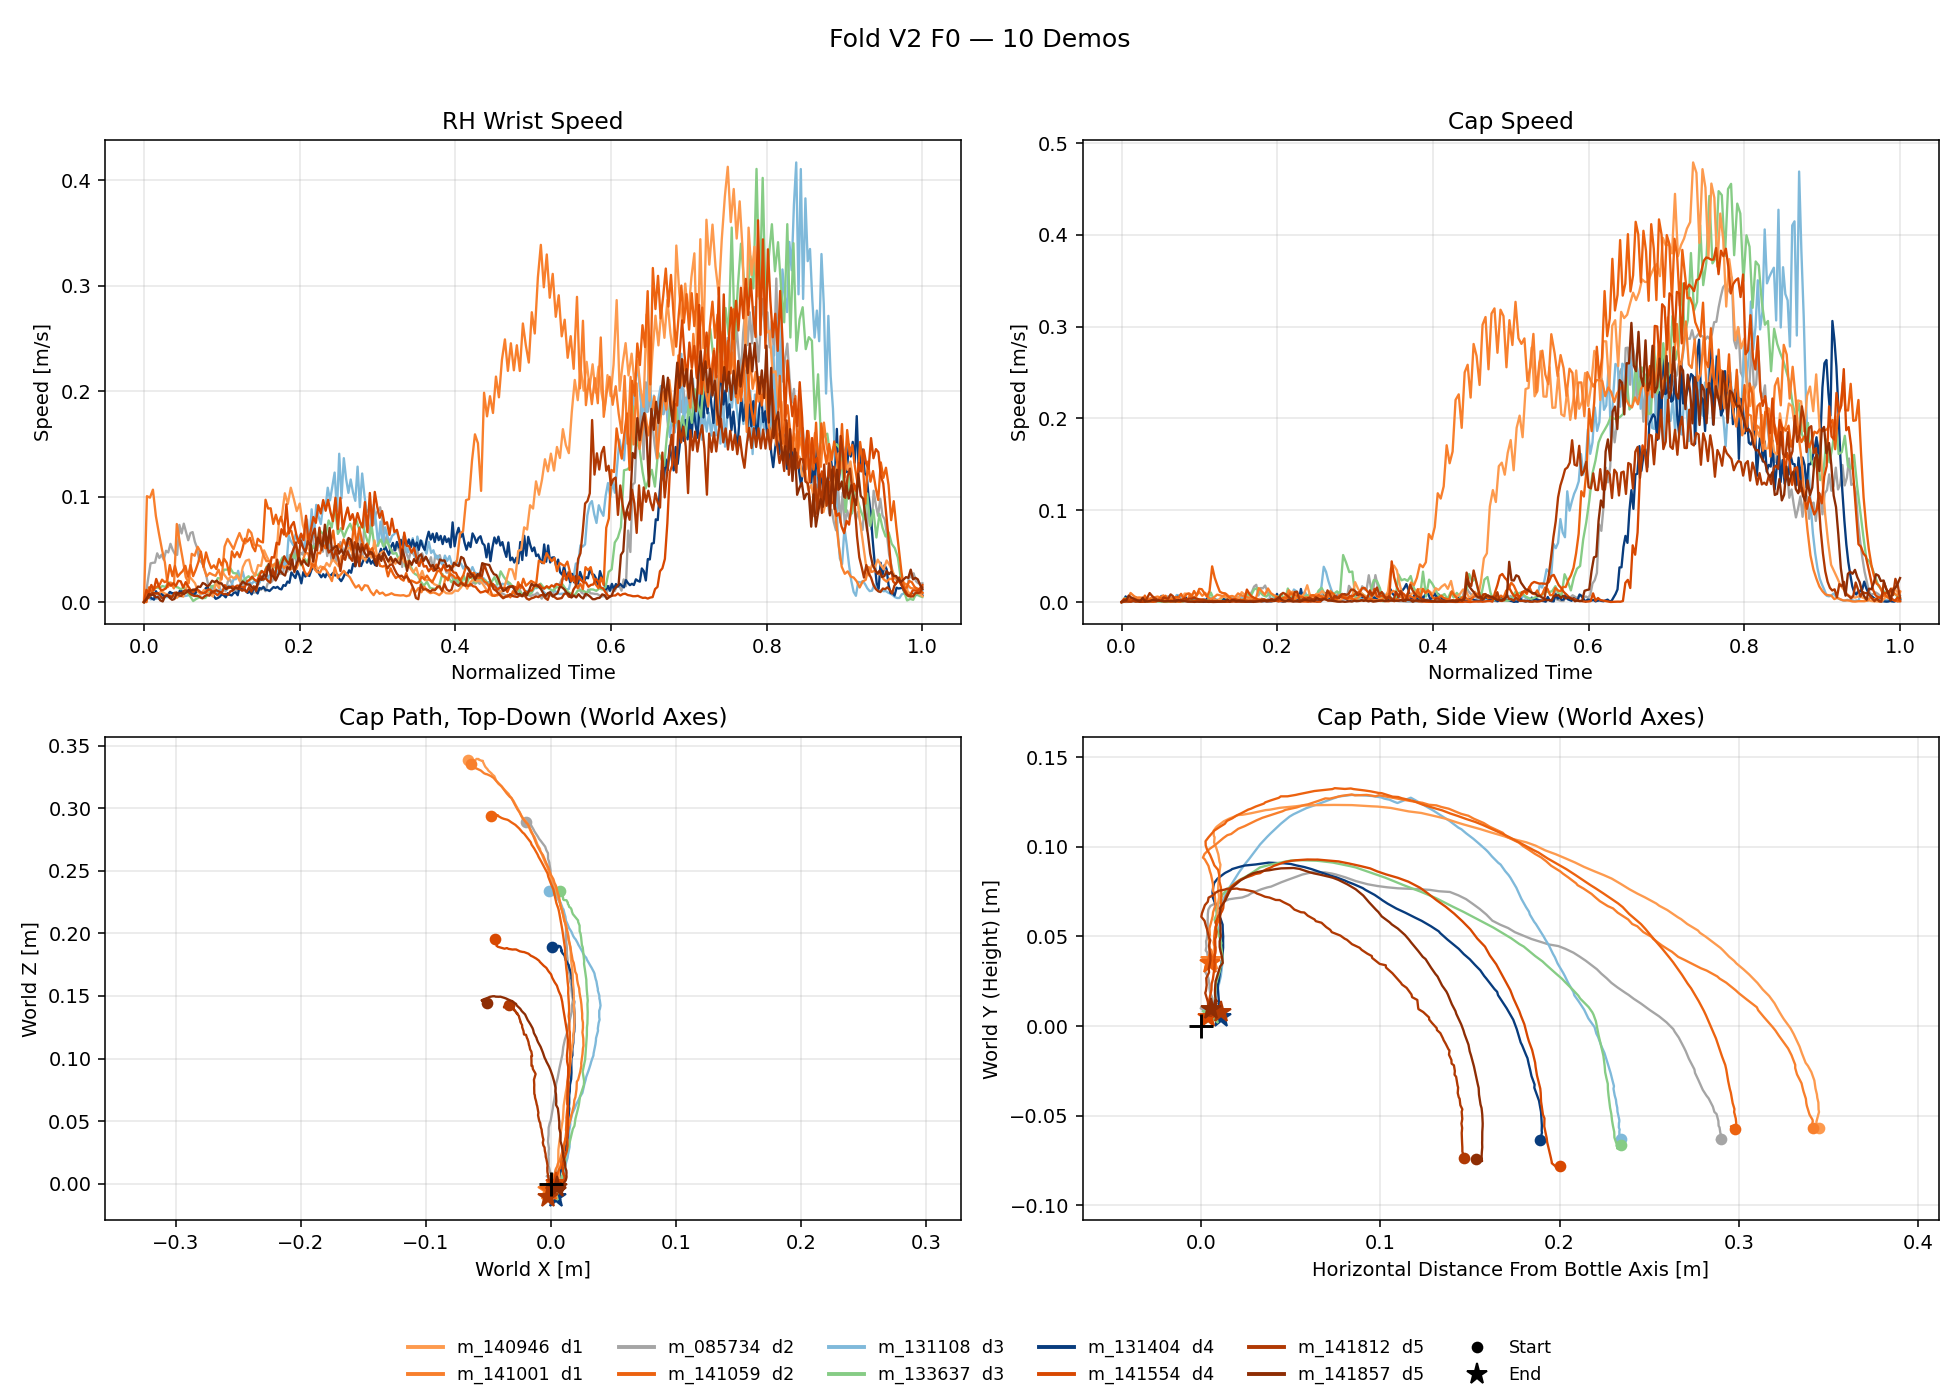
\includegraphics[scale=0.4]{../figures/reach_fold_v2F0.png}
    \caption{Reach demonstrations of cross-validation fold F0 (10 demonstrations, two per reach distance). Top: right-wrist and cap speed against normalized time, computed with the causal estimator used for the training targets. Bottom left: cap path viewed from above, expressed in world axes about the burner. Bottom right: the same paths as horizontal distance from the burner axis against height. Color denotes capture session; markers indicate the start (circle) and end (star) of each trajectory.}
    \label{fig:fold_demo_distribution}
\end{figure}

\paragraph{Velocity estimation.}
Reference velocities are computed with the same estimator used to generate the tracking
targets at training time, so that the quantities plotted are exactly those the policy is
required to reproduce. Linear velocities follow the causal \texttt{pos\_ema} branch of the
demonstration loader: the position signal is first low-pass filtered with a forward-only
exponential moving average, seeded at the initial sample,
%
\begin{equation}
  \tilde{p}[t] = \alpha\, p[t] + (1-\alpha)\, \tilde{p}[t-1],
  \qquad \tilde{p}[0] = p[0], \qquad \alpha = 0.3 ,
  \label{eq:causal-ema}
\end{equation}
%
and the smoothed signal is then differenced backward in time,
%
\begin{equation}
  v[t] = \frac{\tilde{p}[t] - \tilde{p}[t-1]}{\Delta t},
  \qquad v[0] = 0, \qquad \Delta t = \tfrac{1}{60}\,\mathrm{s} ,
  \label{eq:backward-diff}
\end{equation}
%
where $\Delta t$ is the nominal capture period rather than the measured timestamps.
Smoothing prior to differentiation avoids amplifying measurement noise through the
derivative, which occurs if the velocity itself is filtered instead. The estimator uses only
past and current frames and therefore never anticipates the trajectory; it is realizable in
real time and reproduces the output of the live streaming interface, so an offline
demonstration target is identical to the signal that would be observed online at the same
instant. A non-causal alternative (central differences followed by Gaussian smoothing)
yields a cleaner but unrealizable signal and is not used here. One consequence for the
interpretation of the speed panels is that the plotted curves carry the phase lag of the
causal filter: they represent the velocities the policy is asked to track, not an idealized
estimate of the demonstrator's motion.

\paragraph{Spatial organization of the demonstrations.}
The lower panels show the cap trajectory relative to the burner, subtracting its position but retaining world axes. The burner is approximately rotationally symmetric about its vertical axis, so the yaw the motion-capture system assigns it is a marker-placement artifact that varies across sessions; dividing it out would rotate each demonstration by an arbitrary amount. Its body-local vertical also departs from true vertical by several degrees in some captures, which would bias the measured height. The demonstrations form a radial ladder: the cap begins $0.343$, $0.294$, $0.234$, $0.195$ and $0.150$~m from the burner for \texttt{d1}--\texttt{d5}, spaced by approximately $5$~cm, with the two takes of each condition agreeing to within $11$~mm, and all trajectories rise and converge on the origin, where the cap is seated. Start positions are not confined to a single approach ray: initial approach angles span $88.2^\circ$--$109.6^\circ$ and lateral offsets $-0.066$ to $+0.008$\,m, varying within a condition as well as between conditions (d4 differs by $13.1^\circ$, d5 by $6.3^\circ$, d1 by only $0.2^\circ$). This scatter was introduced deliberately during capture so that the policy would observe a range of approach angles at every reach distance rather than a single memorized path, complementing the synthetic trajectory augmentation that perturbs the same degree of freedom further.

 
\subsubsection{Observation space}

Observations are a dictionary of three groups, built per hand and concatenated for the bimanual
policy. \texttt{proprioception} and \texttt{privileged} are pure live simulator state --- where the
robot and object \emph{are}; \texttt{target} carries the demonstration intent --- where they
\emph{should be} one step ahead --- with the $\delta$-prefixed entries being the difference between
the two. The one exception is \texttt{object-to-joint distances}, a live contact-affordance feature
grouped with \texttt{target} because it is read by the residual policy alone, not because it carries
demonstration intent. \Cref{tab:obs-space} lists the layout for the Inspire hand ($n_d = 12$
actuated joints, $n_b = 18$ rigid bodies, $5$ contact links --- thumb distal plus four intermediate
phalanges).
\begin{table}[H]
  \centering
  \small
  \setlength{\tabcolsep}{4pt}
  \begin{tabular}{@{}llrrc@{}}
    \toprule
    Group & Component & Symbolic & Dim & Source \\
    \midrule
    \multirow{5}{*}{\texttt{proprioception}}
      & joint positions $q$                    & $n_d$          &  12 & Sim \\
      & $\cos q$, $\sin q$                     & $2n_d$         &  24 & Sim \\
      & wrist position (zeroed)                & $3$            &   3 & --- \\
      & wrist orient., lin./ang.\ velocity     & $10$           &  10 & Sim \\
    \cmidrule(l){2-5}
      & \emph{subtotal}                        & $13 + 3n_d$    & \textbf{49} & \\
    \midrule
    \multirow{7}{*}{\texttt{privileged}}
      & joint velocities $\dot{q}$             & $n_d$          &  12 & Sim \\
      & object position (wrist frame), quat.   & $7$            &   7 & Sim \\
      & object lin./ang.\ velocity             & $6$            &   6 & Sim \\
      & contact-link force $+$ magnitude       & $5\times4$     &  20 & Sim \\
      & object CoM (wrist frame)               & $3$            &   3 & Sim\,$+$\,Static \\
      & object weight                          & $1$            &   1 & Static \\
    \cmidrule(l){2-5}
      & \emph{subtotal}                        & $n_d + 37$     & \textbf{49} & \\
    \midrule
    \multirow{7}{*}{\texttt{target}}
      & wrist pose target$^{\dagger}$          & $23$           &  23 & AVP \\
      & joint pos.\ target$^{\ddagger}$        & $9(n_b\!-\!1)$ & 153 & AVP \\
      & object pose target$^{\dagger}$         & $23$           &  23 & OT \\
      & object-to-joint distances              & $n_b$          &  18 & Sim \\
      & ref.\ fingertip--object distances      & $5$            &   5 & AVP\,$+$\,OT \\
      & object shape encoding (BPS)            & $128$          & 128 & Static \\
    \cmidrule(l){2-5}
      & \emph{subtotal}                        & $170 + 10n_b$  & \textbf{350} & \\
    \midrule
    \multicolumn{2}{@{}l}{\textbf{Total, per-hand policy input}}  & & \textbf{448} & \\
    \multicolumn{2}{@{}l}{\textbf{Total, bimanual policy input}}  & & \textbf{896} & \\
    \bottomrule
  \end{tabular}
   \caption{Per-hand observation space for the Inspire hand. 
  $^{\dagger}\delta$pos, vel, $\delta$vel, quat, $\delta$quat, $\omega$, $\delta\omega$.
  $^{\ddagger}\delta$pos, vel, $\delta$vel per non-base link. $\delta$ = demonstration minus
  simulation. \textbf{Source}: Sim = live PhysX state; AVP = Apple Vision Pro
  hands; OT = OptiTrack objects, Static = object-model constant.}
  \label{tab:obs-space}
\end{table}

\subsection{Data Augmentation}
\label{sec:augmentation}

Each demonstration is a per-hand trajectory of wrist pose, $21$ MANO keypoints, object pose, and
the corresponding linear and angular velocities over $T$ frames. All spatial augmentations are
yaw-only rotations about the world $Z$ axis, so the direction of gravity and the contact with the
table remain physically consistent. Each augmentation is the same rigid map applied about a
(possibly time-varying) pivot $c_t$:
%
\begin{equation}
  p_t \;\mapsto\; R\,(p_t - c_t) + c_t,
  \qquad
  q_t \;\mapsto\; R\,q_t,
  \qquad
  \dot{p}_t \;\mapsto\; R\,(\dot{p}_t - \dot{c}_t) + \dot{c}_t,
  \qquad
  \omega_t \;\mapsto\; R\,\omega_t ,
  \label{eq:aug-map}
\end{equation}
%
where $R = R_z(\theta)$. The velocity carries the $\dot{c}_t$ correction because the pivot itself
moves with the object. The variants differ only in \emph{which bodies are transformed} and
\emph{what serves as the pivot}; they are summarized in \Cref{tab:augmentations}.

\newcolumntype{Y}{>{\raggedright\arraybackslash}X}

\begin{table}[t]
  \centering
  \small
  \caption{Demonstration augmentations. All rotations are about the world $Z$ axis. LH and RH
  denote the left and right hand demonstration (hand plus the object it manipulates).}
  \label{tab:augmentations}
  \begin{tabularx}{\linewidth}{@{}l Y Y Y@{}}
    \toprule
    Augmentation & Bodies moved & Pivot $c_t$ & Angle \\
    \midrule
    RH about LH object & RH hand + RH object & LH object center, \newline per frame
      & $\mathcal{U}(-15^\circ, +15^\circ)$, constrained \\
    RH about RH object & RH hand (object spins in place) & RH object center, \newline per frame
      & $\mathcal{U}(-15^\circ, +30^\circ)$ \\
    LH about LH object & LH hand + LH object (rigidly) & LH object center, \newline per frame
      & $\mathcal{U}(-15^\circ, +30^\circ)$ \\
    Object yaw & object orientation only & object's own center
      & $\mathcal{U}(-90^\circ, +90^\circ)$, per hand \\
    Keypoint noise & wrist + MANO joints & ---
      & additive $\mathcal{U}(-\sigma, +\sigma)$ \\
    \bottomrule
  \end{tabularx}
\end{table}

\paragraph{Augmentation Types}
\begin{itemize}
  \item \textbf{RH about LH object} is the only augmentation that varies the \emph{inter-hand}
        geometry, letting the right hand approach the object held by the left hand from a different
        direction. This is the coordination variable the residual policy must generalize over in
        the capping task.
  \item \textbf{RH about RH object} orbits the right hand around the object it already holds,
        leaving that object's position unchanged, and so varies the grasp approach angle only.
  \item \textbf{LH about LH object} rotates hand and object together, preserving the demonstrated
        grasp and changing only the pose at which the left object is presented.
  \item \textbf{Object yaw} rotates the object's orientation while leaving the hand fixed,
        deliberately breaking the demonstrated grasp alignment so that the policy must cope with an
        object presented at an unseen yaw.
  \item \textbf{Keypoint noise} emulates hand-pose-estimator and motion-capture error, with
        $\sigma$ specified in centimeters; the finger failure thresholds are loosened by a matching
        factor to compensate.
\end{itemize}

\paragraph{Constrained sampling for the RH-about-LH-object rotation.}
The displacement this rotation induces on the starting pose is
%
\begin{equation}
  \Delta x(\theta) \;=\; \bigl| (\cos\theta - 1)\, u_x \;-\; \sin\theta\; u_y \bigr| ,
  \qquad u = p_0 - c_0 ,
  \label{eq:start-shift}
\end{equation}
%
i.e.\ linear in the initial lever arm $u$. A single scene-wide angle therefore displaces a
demonstration that begins far from the left object much further than one that begins close to it.
The yaw is consequently drawn \emph{per demonstration} by rejection sampling from a symmetric
range, keeping the first draw whose starting displacement satisfies $\Delta x \leq \delta_{\max}$
with $\delta_{\max} = 5\,\mathrm{cm}$. Only the start is bounded; the trajectory is free to diverge
further later, which is what gives the augmentation its effect.

\paragraph{Random action masking}
Following~\cite{teledexter}, a randomly chosen subset of joints is periodically frozen at its previously commanded target, so that the policy cannot assume that every degree of freedom
responds on schedule. This is the only augmentation acting on the \emph{action} channel rather than on the
observation. At each control step, an environment with no active mask starts one with probability
$p$; a fresh mask selects $n$ degrees of freedom per hand uniformly without replacement and holds
them for $d \sim \mathcal{U}\{1, d_{\max}\}$ steps. The masking is applied \emph{after} the action
moving average and joint-limit clamp, so what is frozen is the final commanded joint target, and
the held value is written back as the previous target so that a multi-step freeze holds one command
throughout rather than drifting. The maximum freeze duration $d_{\max}$ is annealed over
$T_{\text{ramp}}$ control steps,
%
\begin{equation}
  \sigma(t) = 1 - (1 - \sigma_{\min})\min\!\left(\tfrac{t}{T_{\text{ramp}}}, 1\right),
  \qquad
  d_{\max}(t) = 1 + (D_{\max} - 1)\,\frac{1 - \sigma(t)^3}{1 - \sigma_{\min}^3},
  \qquad \sigma_{\min} = 0.7 ,
  \label{eq:mask-ramp}
\end{equation}
%
so the policy is always exposed to brief stale commands early in training; as $d_{\max}$ grows, single-step freezes continue to occur at full frequency while the mean freeze duration increases. Masks are drawn independently at each control step, so at any instant the batch spans a spectrum of partially stale joint commands; they are cleared on reset so a fresh episode never inherits one.

\paragraph{Hyperparameters}
The policy is an encoder followed by a shared actor--critic trunk. The encoder concatenates the three observation groups (\Cref{tab:obs-space}) and compresses the resulting $896$-d vector to a $256$-d latent through a three-hidden-layer MLP of width $512$ with Swish activations. The two frozen imitators' base actions are appended to this latent rather than passed through the encoder, so the residual sees them at full resolution; the resulting $292$-d feature is processed by a four-layer trunk of widths $[256, 512, 128, 64]$ with ELU activations, shared between the policy and value heads. Two linear heads emit the action mean and the state value, with a state-independent learned log-standard-deviation. Full hyperparameters are listed in \Cref{tab:policy-hparams}.

\begin{table}[H]
  \centering
  \small
  \begin{tabular}{@{}ll@{}}
    \toprule
    Hyperparameter & Value \\
    \midrule
    \multicolumn{2}{@{}l}{\textit{Network}} \\
    Encoder hidden sizes            & $[512, 512, 512]$ \\
    Encoder output dim              & $256$ \\
    Encoder activation              & Swish \\
    MLP hidden sizes                & $[256, 512, 128, 64]$ \\
    Activation                      & ELU \\
    \midrule
    \multicolumn{2}{@{}l}{\textit{PPO}} \\
    Learning rate                   & $2 \times 10^{-4}$ \\
    LR schedule                     & warm-up, then adaptive \\
    KL threshold                    & $0.008$ \\
    Num opt-epochs                  & $5$ \\
    Minibatch size                  & $4{,}096$ \\
    Horizon length                  & $32$ \\
    Discount ($\gamma$)             & $0.99$ \\
    GAE $\lambda$                   & $0.95$ \\
    Clip range ($\epsilon$)         & $0.2$ \\
    Max grad norm                   & $1.0$ \\
    Bounds-loss coef.               & $10^{-4}$ \\
    Parallel envs                   & $8{,}192$ \\
    \bottomrule
  \end{tabular}
  \caption{Hyperparameters of the residual policy.}
  \label{tab:policy-hparams}
\end{table}